\documentclass[../main.tex]{subfiles}

\begin{document}

\section{Theory}\label{sec:theory}

\subsection{Franke's function}
Franke's function is a function which is often used to test different regression and interpolation methods. The function has two Gaussian peaks of differing heights, and a smaller dip. It's expression is

\begin{align*}
  f(x,y) &= \frac{3}{4}\exp{\left(-\frac{(9x-2)^2}{4} - \frac{(9y-2)^2}{4}\right)}+\frac{3}{4}\exp{\left(-\frac{(9x+1)^2}{49}- \frac{(9y+1)}{10}\right)} \\
  &+\frac{1}{2}\exp{\left(-\frac{(9x-7)^2}{4} - \frac{(9y-3)^2}{4}\right)} -\frac{1}{5}\exp{\left(-(9x-4)^2 - (9y-7)^2\right) }.
\end{align*}

and we define it for the interval $x,y\in[0,1]$. An illustration of Franke's function can be seen in figure \ref{fig:frankesplot}

\begin{figure}
  \centering
  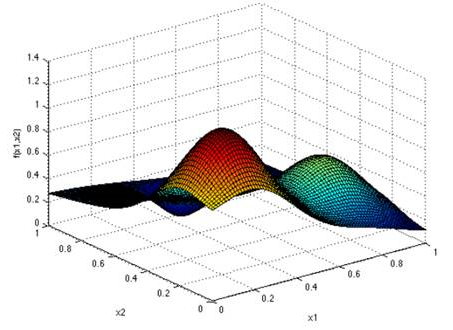
\includegraphics[width = 3in]{frankesfunction_plot.png}
  \caption{Shape of Franke's function which will be used as a interpolating goal.
  \\Note to self: Might be better to plot the graph instead of using a figure from the web. Remember to add the source for the figure by using for example bib. https://www.sfu.ca/~ssurjano/franke2d.html}
  \label{fig:frankesplot}
\end{figure}

\subsubsection{The Vandermonde matrix applied to Franke's function}

When performing the different regression methods, it is important to sort the data into a well designed system for easy access and easier calculations. The data which is to be used during the calculations is sorted into a so called Vandermonde matrix, which is also known as a design matrix. A Vandermonde matrix is a matrix where the rows is built up by geometric progression \cite{vandermonde}.\\

Franke's function is a two dimensional function defined by the components x and y. Then it is instinctive to have a design matrix X also built up by x and y components into a $n\cross p$ matrix, the following way

\[
\begin{array}{lcccccc}
  \verb|X=| & \left(\begin{array}{@{}ccccccc@{}}
    x_0 & y_0 & x_0^2 & x_0y_0 & y_0^2 & \ldots & x_0^d y_0^{p-d}\\
    x_1 & y_1 & x_1^2 & x_1y_1 & y_1^2 & \ldots & x_1^d y_1^{p-d}\\
     &  &  &  &  & \vdots & \\
    x_{n-1} & y_{n-1} & x_{n-1}^2 & x_{n-1}y_{n-1} & y_{n-1}^2 & \ldots & x_{n-1}^d y_{n-1}^{p-d}\\
 \end{array}\right) \\[15pt]
\end{array}
\]

Where the d is the degree of polynomial. Making the degree higher leads to more complicated equations which naturally gives a more precise regression. Having a design matrix built up by too many terms per polynomial increases the possibility of eventually getting an over fitting model, which will be discussed later in the article.\\

By having different weights $\Beta$ in front of each term in the design matrix, it is possible to calculate how large each term in the polynomials should be in order to make the best approximation. This is the clue of having a design matrix built up by x and y components, making it possible to approximate the polynomials which will fit the Franke's function best. Then the approximation can be written as the following

\begin{equation}
    \tilde{y}=X\beta+\epsilon
\end{equation}

Where $\epsilon$ is the error. This can be written as

\[
\begin{array}{lccccccc}
  \verb|\tilde{y}=| & \left(\begin{array}{@{}cccccccc@{}}
    \epsilon_0 & \beta_0 x_0 &  \beta_1 y_0 &  \beta_2 x_0^2 &  \beta_3 x_0y_0 &  \beta_4 y_0^2 & \ldots &  \beta_5 x_0^d y_0^{p-d}\\
    \epsilon_1 & \beta_0 x_1 &  \beta_1 y_1 &  \beta_2 x_1^2 &  \beta_3 x_1y_1 &  \beta_4 y_1^2 & \ldots &  \beta_5 x_1^d y_1^{p-d}\\
     &  &  &  &  & \vdots & \\
    \epsilon_{n-1} & \beta_0 x_{n-1} & \beta_1 y_{n-1} & \beta_2 x_{n-1}^2 & \beta_3 x_{n-1}y_{n-1} & \beta_4 y_{n-1}^2 & \ldots & \beta_5 x_{n-1}^d y_{n-1}^{p-d}\\
 \end{array}\right) \\[15pt]
\end{array}
\]



\begin{comment}
Reference to be added to the bib file:
\end{comment}



\subsection{Linear regression}
The goal of a linear regression model is to find the coefficients $\hat{\mathbf \beta}$ best suited for predicting new data via this expression:

\begin{equation*}
  \hat{\mathbf y} = \mathbf X\hat{\mathbf \beta},
\end{equation*}

where $\mathbf X$ is the design matrix constructed from the input data, and $\hat{\mathbf y}$ is the resulting prediction. To achieve this, we define a "cost function" of sorts, that evaluates each coefficients ability to predict the initial training dataset. We then find the $\hat{\mathbf \beta}$ that minimizes this cost function. More formally put, we want to find

\begin{equation}
  \hat{\mathbf \beta} = \underset{\beta}{\arg \min}\ C(\beta),
\end{equation}

where $C(\beta)$ is the cost function.


\subsubsection{Ordinary least squares regression ($L_0$)}
Ordinary least squares (OLS) regression uses the residual sum of squares (RSS) function as the cost function. Given $N$ datapoints and the predicted output $\mathbf y$, it reads

\begin{equation}
  \label{eq:rss}
  \text{RSS}(\beta) = \sum_{i=1}^N (y_i - \hat y_i)^2.
\end{equation}

As found in \hyperref[sec:L0_matrix_form]{appendix \ref*{sec:L0_matrix_form}}, a cost function like (\ref{eq:rss}) gives the following matrix equation for $\hat{\mathbf \beta}$

\begin{equation}
  \label{eq:L0_matrix_form}
  \hat \beta = (\mathbf X^T\mathbf X)^{-1}\mathbf X^T \mathbf y
\end{equation}

OLS regression has very low variance, but high bias - as a consequence of the bias-variance tradeoff. This makes OLS regression an "accurate" predictor of its own training data, but susceptible to overfitting, which the following two models are better suited to handle.


\subsubsection{Lasso regression ($L_1$)}
Lasso regression expands upon the above cost function by adding a term that penalizes the size of each coefficient. This is done by a factor of $\lambda$, as shown here:

\begin{equation}
  \label{eq:L1_algo}
  \hat{\mathbf \beta} = \underset{\beta}{\arg \min} \begin{Bmatrix}\sum_{i=1}^N\left(y_i - \beta_0 - \sum_{j=1}^p x_{ij}\beta_j\right)^2 + \lambda \sum_{j=1}^p |\beta_j| \end{Bmatrix} .
\end{equation}

The first sum is from the RSS function, while the second sum is the imposed penalty. The Lasso decreases bias from the OLS model, by decreasing the size of the coefficients, and thus making the variables more equally weighted. \\

Lasso regression has no closed form expression for $\hat{\mathbf \beta}$, which means it must be calculated programatically.


\subsubsection{Ridge regression ($L_2$)}
Ridge regression has a penalty corresponding to the coefficient's squared sizes, further decreasing the bias from The Lasso, but obviously also increases variance. It defines $\hat{\mathbf \beta}$ like this

\begin{equation*}
  \hat \beta^{\text{ridge}} = \underset{\beta}{\arg \min} \begin{Bmatrix}\sum_{i=1}^N\left(y_i - \beta_0 - \sum_{j=1}^p x_{ij}\beta_j\right)^2 + \lambda \sum_{j=1}^p \beta_j^2 \end{Bmatrix},
\end{equation*}

which - by the same proceedure as shown in \hyperref[sec:L0_matrix_form]{appenix \ref*{sec:L0_matrix_form}}, has this closed form expression

\begin{equation}
  \hat \beta^{\text{ridge}} = (\mathbf X^T\mathbf X + \lambda \mathbf I)^{-1}\mathbf X^T\mathbf y.
\end{equation}

\end{document}
